\documentclass[11pt]{article} % use larger type; default would be 10pt

\usepackage{pgfplots}
\usetikzlibrary{calc}
\usetikzlibrary{arrows}
\usetikzlibrary{patterns}
\usetikzlibrary{calc,intersections,through,backgrounds}
\usetikzlibrary{decorations.pathreplacing}
        \newcommand\degree[0]{^{\circ}}
        \newcommand\abs[1]{\left|#1\right|}

\title{Play with TikZ}
\author{Just Us}
%\date{} % Activate to display a given date or no date (if empty),
         % otherwise the current date is printed 

\begin{document}
\maketitle

\section{Chap 9 Vectors}

\subsection{9.1 Geometric form}

exam9-1-1a campsite position vector

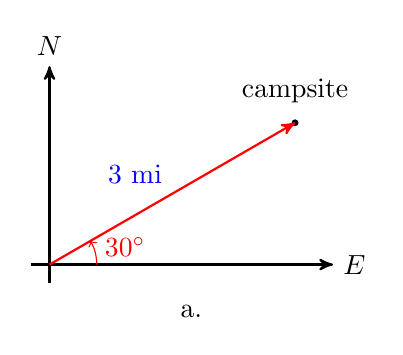
\begin{tikzpicture} [scale=1.2]
\coordinate (O) at (0,0);
\coordinate (P) at (30:3);
\draw[black,thick,->,>=stealth'] (-.2,0)--(3,0) node[right]{$E$};
\draw[black,thick,->,>=stealth'] (0,-.2)--(0,2.1) node[above]{$N$};
\filldraw[black] (P) circle (.03cm) node[yshift=.4cm]  {campsite};
\draw[red,thick,->,>=stealth'] (O)--(P) node[above left, midway, text=blue]{3 mi};
\draw[red,->] (0.5,0) arc(0:30:.5) node[right, yshift=2,midway] {$30\degree$};
\node at (1.5,-.5) {a.};
\end{tikzpicture}
\newline

exam9-1-1b wind-velocity vector

\begin{tikzpicture} [scale=.12]
\coordinate (O) at (0,0);
\coordinate (P) at (180:50);
\draw[black,thick,->,>=stealth'] (0,0)--(10,0) node[right]{$E$};
\draw[black,thick,->,>=stealth'] (0,-2)--(0,20) node[above]{$N$};
\filldraw[black] (P) circle (.03cm) node[left]  {$W$};
\draw[red,thick,->,>=stealth'] (O)--(P) node[above , midway, text=blue]{50 km/hr};
\draw[red,->] (3,0) arc(0:180:3) node[above right, yshift=-2,midway] {$180\degree$};
\node at (-20,-5) {b.};
\end{tikzpicture}
\newline

exer9-1-1ans airplne velocity vector

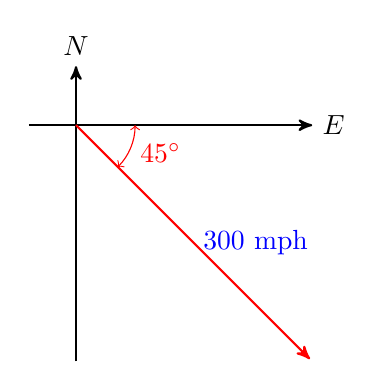
\begin{tikzpicture} [scale=1.5]
\coordinate (O) at (0,0);
\coordinate (P) at (-45:2.8);
\draw[black,thick,->,>=stealth'] (-.4,0)--(2,0) node[right]{$E$};
\draw[black,thick,->,>=stealth'] (0,-2)--(0,.5) node[above]{$N$};
\draw[red,thick,->,>=stealth'] (O)--(P) node[right, midway, text=blue]{300 mph};
\draw[red,<->] (0.5,0) arc(0:-45:.5) node[right, yshift=-2,midway] {$45\degree$};
\end{tikzpicture}
\newline

fig9-1-1 vectors

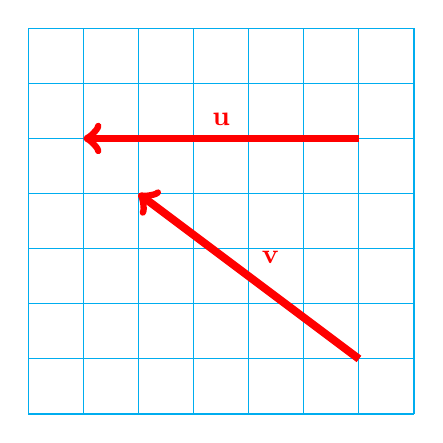
\begin{tikzpicture} [scale=.7]
\draw[cyan] (0,0) grid (7,7);
\draw[red,line width=1.mm, ->] (6,5)--(1,5) node[above,midway] {\textbf{u}};
\draw[red,line width=1.mm, ->] (6,1)--(2,4) node[above right,midway] {\textbf{v}};
\end{tikzpicture}
\newline

exam9-1-2 vectors

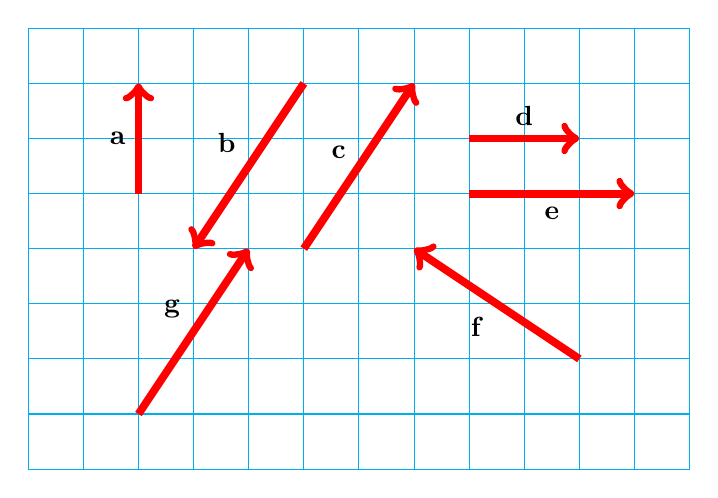
\begin{tikzpicture} [scale=.7]
\draw[cyan] (0,0) grid (12,8);
\draw[red,line width=1.mm, ->] (2,5)--++(0,2) node[left,midway, text=black] {\textbf{a}};
\draw[red,line width=1.mm, ->] (5,7)--++(-2,-3) node[above left,midway, text=black] {\textbf{b}};
\draw[red,line width=1.mm, <-] (7,7)--++(-2,-3) node[above left, yshift=-2,midway, text=black] {\textbf{c}};
\draw[red,line width=1.mm, ->] (8,6)--++(2,0) node[above,midway, text=black] {\textbf{d}};
\draw[red,line width=1.mm, ->] (8,5)--++(3,0) node[below,midway, text=black] {\textbf{e}};
\draw[red,line width=1.mm, ->] (10,2)--++(-3,2) node[below left,midway, text=black] {\textbf{f}};
\draw[red,line width=1.mm, ->] (2,1)--++(2,3) node[above left,midway, text=black] {\textbf{g}};
\end{tikzpicture}
\newline

exer9-1-2 vector

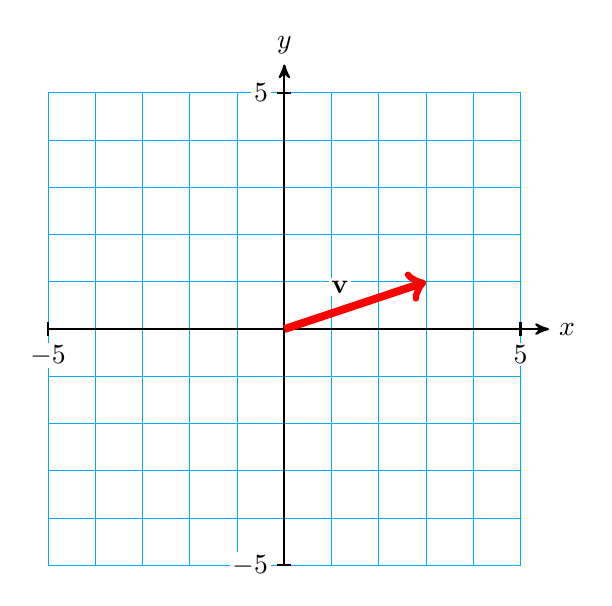
\begin{tikzpicture} [scale=.6]
\draw[cyan] (-5,-5) grid (5,5);
\draw[black,thick,->,>=stealth'] (-5,0)--(5.6,0) node[right] {$x$};
\draw[black,thick,->,>=stealth'] (0,-5)--(0,5.6) node[above] {$y$};
\draw[red,line width=1.mm, ->] (0,0)--++(3,1) node[above left,midway,yshift=2, fill=white, inner sep=1, text=black] {\textbf{v}};
\foreach \x in {-5,5} {
 \draw[black,thick] (\x,.15)--++(0,-.3) node[below, yshift=-2, fill=white, inner sep=1] {$\x$};
 \draw[black,thick] (.15,\x)--++(-.3,0) node[left, xshift=-2, fill=white, inner sep=1] {$\x$};
};
\end{tikzpicture}
\newline


exer9-1-2ans vectors

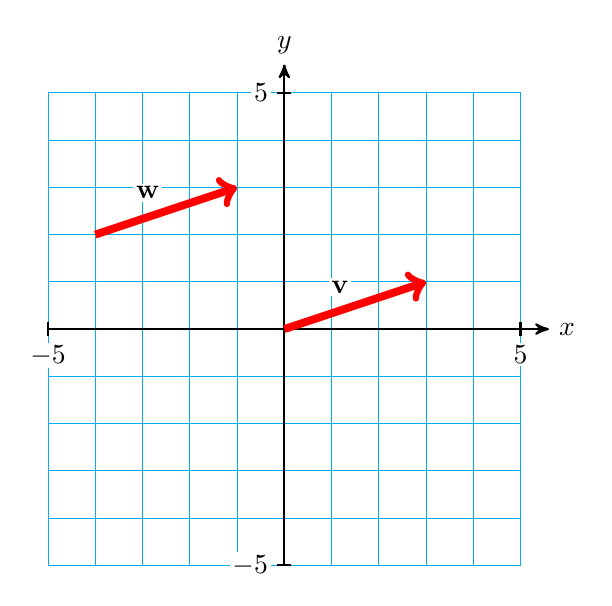
\begin{tikzpicture} [scale=.6]
\draw[cyan] (-5,-5) grid (5,5);
\draw[black,thick,->,>=stealth'] (-5,0)--(5.6,0) node[right] {$x$};
\draw[black,thick,->,>=stealth'] (0,-5)--(0,5.6) node[above] {$y$};
\draw[red,line width=1.mm, ->] (0,0)--++(3,1) node[above left,midway,yshift=2, fill=white, inner sep=1, text=black] {\textbf{v}};
\foreach \x in {-5,5} {
 \draw[black,thick] (\x,.15)--++(0,-.3) node[below, yshift=-2, fill=white, inner sep=1] {$\x$};
 \draw[black,thick] (.15,\x)--++(-.3,0) node[left, xshift=-2, fill=white, inner sep=1] {$\x$};
};
\draw[red,line width=1.mm, ->] (-4,2)--++(3,1) node[above left,midway,yshift=2, fill=white, inner sep=1, text=black] {\textbf{w}};
\end{tikzpicture}
\newline

fig9-1-2 vectors

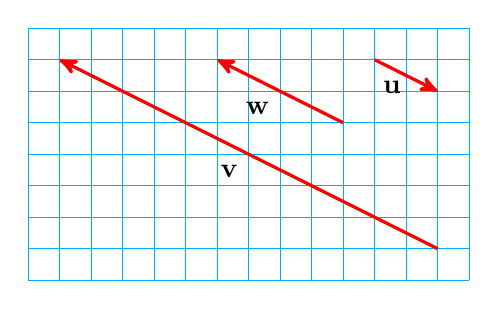
\begin{tikzpicture} [scale=.4]
\draw[cyan] (-7,-4) grid (7,4);
\draw[red, very thick, ->,>=stealth'] (6,-3)--(-6,3) node[below left, midway, text=black]{\textbf{v}};
\draw[red, very thick, ->,>=stealth'] (3,1)--(-1,3) node[below left, midway, text=black]{\textbf{w}};
\draw[red, very thick, ->,>=stealth'] (4,3)--(6,2) node[below left, xshift=2, yshift=2, midway, text=black]{\textbf{u}};
\end{tikzpicture}
\newline

exam9-1-3 two grids of vectors

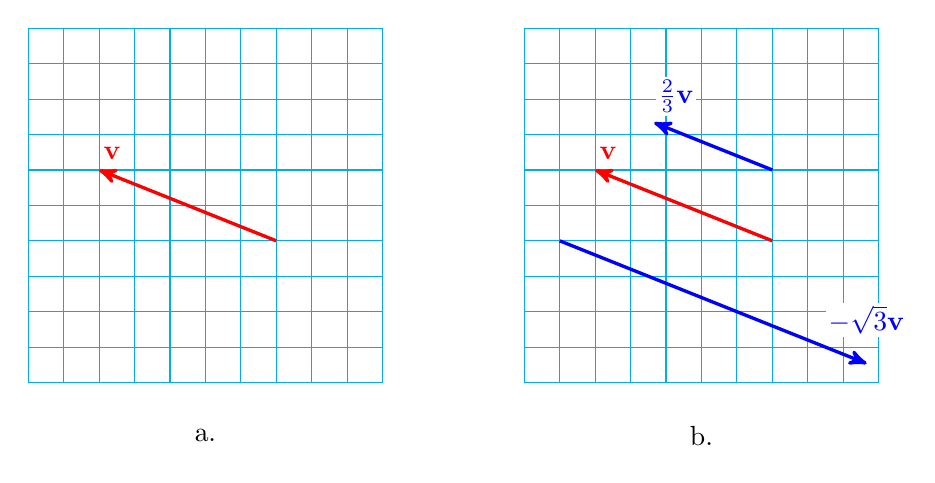
\begin{tikzpicture} [scale=.45]
\draw[cyan] (-5,-5) grid (5,5);
\draw[red, very thick, ->,>=stealth'] (2,-1)--++(-5,2) node[above right, yshift=2, fill=white, inner sep=1] {\textbf{v}};
\node at (0,-6.5) {a.};

\def\xs{14};
\draw[cyan] ($ \xs*(1,0) + (-5,-5)$) grid ($ \xs*(1,0) + (5,5)$);
\draw[red, very thick, ->,>=stealth'] ($ \xs*(1,0) + (2,-1)$)--++(-5,2) node[above right, yshift=2, fill=white, inner sep=1] {\textbf{v}};
\draw[blue, very thick, ->,>=stealth'] ($ \xs*(1,0) + (2,1)$)--++(-10/3,4/3) node[above right, yshift=2, fill=white, inner sep=1] {$\frac{2}{3}$\textbf{v}};
\draw[blue, very thick, ->,>=stealth'] ($ \xs*(1,0) + (-4,-1)$)--++ ($ -sqrt(3)*(-5,0) + -sqrt(3)*(0,2) $) node[above, yshift=9, fill=white, inner sep=1] {$-\sqrt{3}$\textbf{v}};

\node at ($ \xs*(1,0) + (0,-6.5)$) {b.};
\end{tikzpicture}
\newline

exer9-1-3 vector

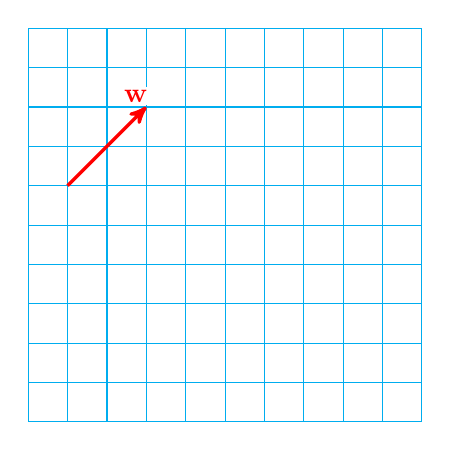
\begin{tikzpicture} [scale=.5]
\draw[cyan] (-5,-5) grid (5,5);
\draw[red, very thick, ->,>=stealth'] (-4,1)--++(2,2) node[above left, xshift=2, fill=white, inner sep=1]{\textbf{w}};
\end{tikzpicture}
\newline

exer9-1-3ans vectors

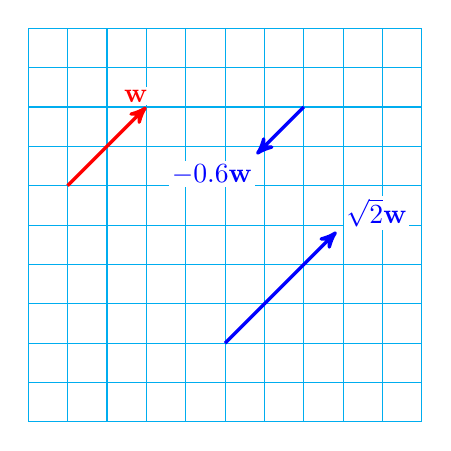
\begin{tikzpicture} [scale=.5]
\draw[cyan] (-5,-5) grid (5,5);
\draw[red, very thick, ->,>=stealth'] (-4,1)--++(2,2) node[above left, xshift=2, fill=white, inner sep=1]{\textbf{w}};
\draw[blue, very thick, ->,>=stealth'] (2,3)--++(-1.2,-1.2) node[below left, yshift=-2, fill=white, inner sep=1]{$-0.6$\textbf{w}};
\draw[blue, very thick, ->,>=stealth'] (0,-3)--++($ sqrt(2)*(2,2) $) node[above right, xshift=2, fill=white, inner sep=1]{$\sqrt{2}$\textbf{w}};
\end{tikzpicture}
\newline


fig9-1-3 add vectors

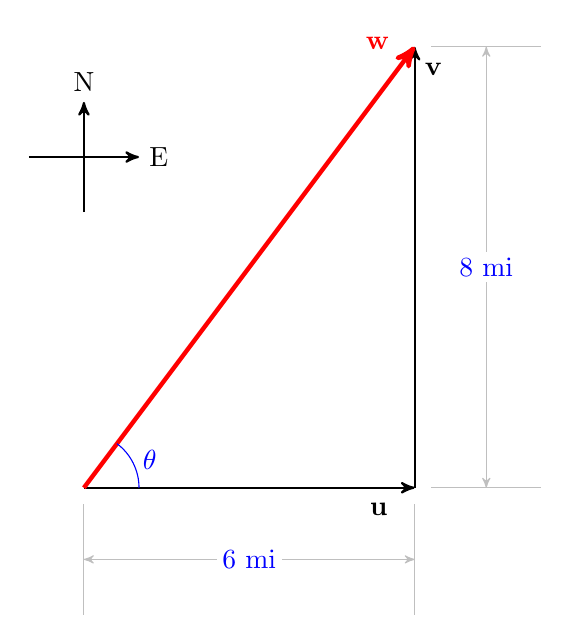
\begin{tikzpicture} [scale=.7]
\coordinate (O) at (0,0);
\coordinate (A) at (6,0);
\coordinate (B) at (6,8);
\draw[black, thick, ->,>=stealth'] (O)--(A) node[below left, xshift=-6, yshift=-2]{\textbf{u}};
\draw[black, thick, ->,>=stealth'] (A)--(B) node[right, yshift=-8]{\textbf{v}};
\draw[red, ultra thick, ->,>=stealth'] (O)--(B) node[above left, xshift=-5, yshift=-5]{\textbf{w}};
\draw[blue] (1,0) arc(0:{atan(4/3)}:1) node[right, yshift=1, midway] {$\theta$};
\draw[black,thick,->,>=stealth'] (-1,6)--++(2,0) node[right]{E};
\draw[black,thick,->,>=stealth'] (0,5)--++(0,2) node[above]{N};
\draw[lightgray] ($ (B) +(0.3,0)$) --++(2,0);
\draw[lightgray] ($ (A) +(0.3,0)$) --++(2,0);
\draw[lightgray, <->,>=stealth'] ($ (B) +(1.3,0)$) --($ (A) +(1.3,0)$) node[midway, text=blue, fill=white, inner sep=2] {8 mi};
\draw[lightgray] (0, -.3) --++(0,-2);
\draw[lightgray] ($ (A) +(0, -.3)$) --++(0,-2);
\draw[lightgray, <->,>=stealth'] (0,-1.3) --++(6,0) node[midway, text=blue, fill=white, inner sep=2] {6 mi};
\end{tikzpicture}
\newline

exam9-1-4 three grids of vectors

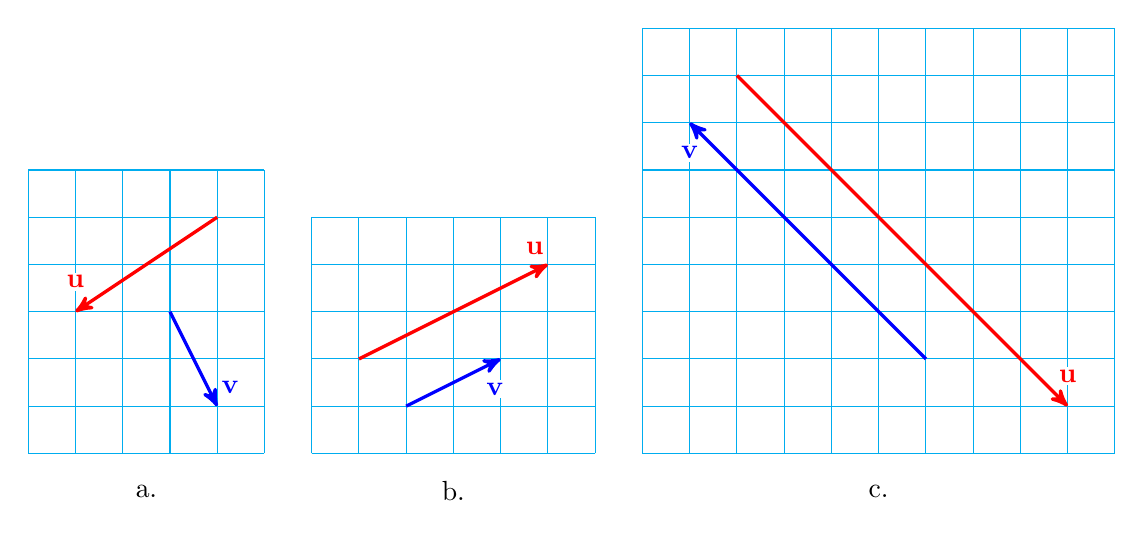
\begin{tikzpicture} [scale=.6]
\coordinate (O) at (0,0);
\draw[cyan] (O) grid ++(5,6);
\draw[red,very thick,->,>=stealth'] ($ (O)+(4,5) $)--++(-3,-2) node[above, yshift=7, fill=white, inner sep=1] {\textbf{u}};
\draw[blue,very thick,->,>=stealth'] ($ (O)+(3,3) $)--++(1,-2) node[above right, yshift=3, fill=white, inner sep=1] {\textbf{v}};
\node at (2.5,-.8) {a.};

\coordinate (O) at (5.999,0);
\draw[cyan] (O) grid ++(6.001,5);
\draw[red,very thick,->,>=stealth'] ($ (O)+(1,2) $)--++(4,2) node[above left, yshift=2, fill=white, inner sep=1] {\textbf{u}};
\draw[blue,very thick,->,>=stealth'] ($ (O)+(2,1) $)--++(2,1) node[below, xshift=-2, yshift=-7, fill=white, inner sep=1] {\textbf{v}};
\node at ($ (O)+(3,-.8)$) {b.};


\coordinate (O) at (12.999,0);
\draw[cyan] (O) grid ++(10,9);
\draw[red,very thick,->,>=stealth'] ($ (O)+(2,8) $)--++(7,-7) node[above , yshift=7, fill=white, inner sep=1] {\textbf{u}};
\draw[blue,very thick,->,>=stealth'] ($ (O)+(6,2) $)--++(-5,5) node[below,  yshift=-7, fill=white, inner sep=1] {\textbf{v}};
\node at ($ (O)+(5,-.8)$) {c.};

\end{tikzpicture}
\newline


exam9-1-4ans three grids of vectors

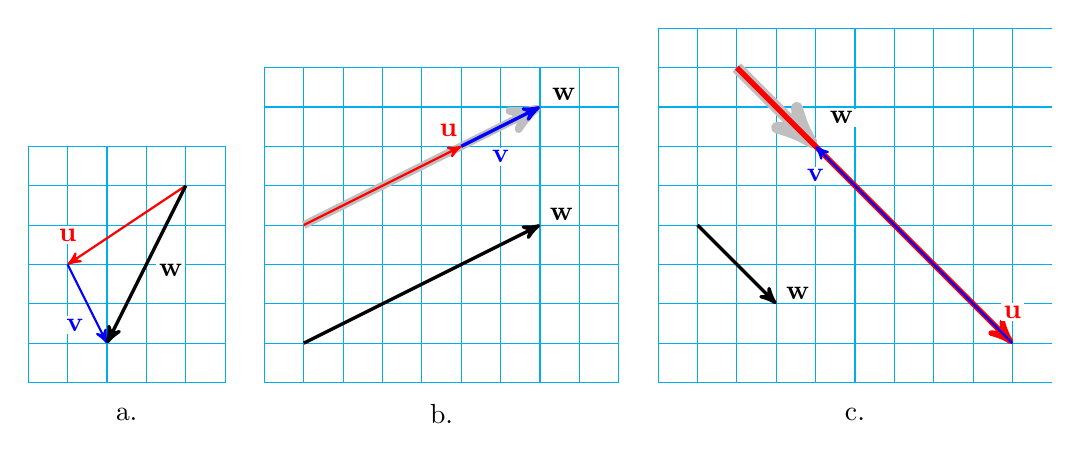
\begin{tikzpicture} [scale=.5]
\coordinate (O) at (0,0);
\draw[cyan] (O) grid ++(5,6);
\draw[red,thick,->,>=stealth'] ($ (O)+(4,5) $)--++(-3,-2) node[above, yshift=7, fill=white, inner sep=1] {\textbf{u}};
\draw[blue,thick,->,>=stealth'] ($ (O)+(1,3) $)--++(1,-2) node[above left, xshift=-7, yshift=3, fill=white, inner sep=1] {\textbf{v}};
\draw[black,very thick,->,>=stealth'] ($ (O)+(4,5) $)--++(-2,-4) node[ right, midway, xshift=3, yshift=-2, fill=white, inner sep=1] {\textbf{w}};
\node at (2.5,-.8) {a.};

\coordinate (O) at (5.999,0);
\draw[cyan] (O) grid ++(9.001,8);
\draw[lightgray,line width=1mm,->,>=stealth'] ($ (O)+(1,4) $)--++(6,3) node[above right, xshift=2, yshift=0, fill=white, inner sep=1, text=black] {\textbf{w}};
\draw[red, thick,->,>=stealth'] ($ (O)+(1,4) $)--++(4,2) node[above left, yshift=2, fill=white, inner sep=1] {\textbf{u}};
\draw[blue,very thick,->,>=stealth'] ($ (O)+(5,6) $)--++(2,1) node[below, midway, xshift=0, yshift=-7, fill=white, inner sep=1] {\textbf{v}};
\draw[black,very thick,->,>=stealth'] ($ (O)+(1,1) $)--++(6,3) node[above right, xshift=2, yshift=0, fill=white, inner sep=1] {\textbf{w}};
\node at ($ (O)+(4.5,-.8)$) {b.};


\coordinate (O) at (15.999,0);
\draw[cyan] (O) grid ++(10,9);
\draw[lightgray,line width=1.5mm,->,>=stealth'] ($ (O)+(2,8) $)--++(2,-2) node[above right, xshift=2, yshift=5, fill=white, inner sep=1, text=black] {\textbf{w}};
\draw[red,line width=.7mm,->,>=stealth'] ($ (O)+(2,8) $)--++(7,-7) node[above , yshift=7, fill=white, inner sep=1] {\textbf{u}};
\draw[blue,thick,->,>=stealth'] ($ (O)+(9,1) $)--++(-5,5) node[below,  yshift=-7, fill=white, inner sep=1] {\textbf{v}};
\draw[black,very thick,->,>=stealth'] ($ (O)+(1,4) $)--++(2,-2) node[above right, xshift=2, yshift=0, fill=white, inner sep=1] {\textbf{w}};
\node at ($ (O)+(5,-.8)$) {c.};

\end{tikzpicture}
\newline

exer9-1-4 two vectors

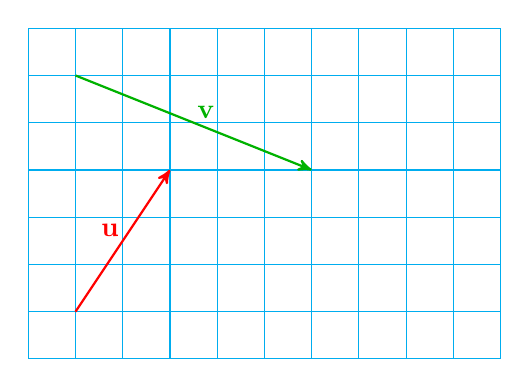
\begin{tikzpicture} [scale=.6]
\draw[cyan] (0,0) grid (10,7);
\draw[red,thick,->,>=stealth'] (1,1) --++(2,3) node[above left, midway, fill=white, inner sep=1] {\textbf{u}};
\draw[green!70!black,thick,->,>=stealth'] (1,6)--++(5,-2) node[above right, midway, fill=white, inner sep=1] {\textbf{v}};

\end{tikzpicture}
\newline

exer9-1-4ans three vectors

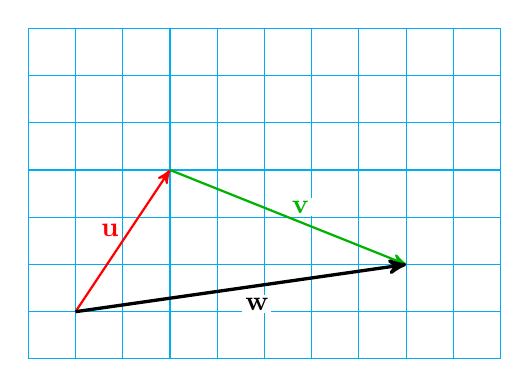
\begin{tikzpicture} [scale=.6]
\draw[cyan] (0,0) grid (10,7);
\draw[red,thick,->,>=stealth'] (1,1) --++(2,3) node[above left, midway, fill=white, inner sep=1] {\textbf{u}};
\draw[green!70!black,thick,->,>=stealth'] (3,4)--++(5,-2) node[above right, midway, fill=white, inner sep=1] {\textbf{v}};
\draw[black,very thick,->,>=stealth'] (1,1) --++(7,1) node[below right, midway, yshift=-2, fill=white, inner sep=1] {\textbf{w}};

\end{tikzpicture}
\newline


exam9-1-5 displacement vectors

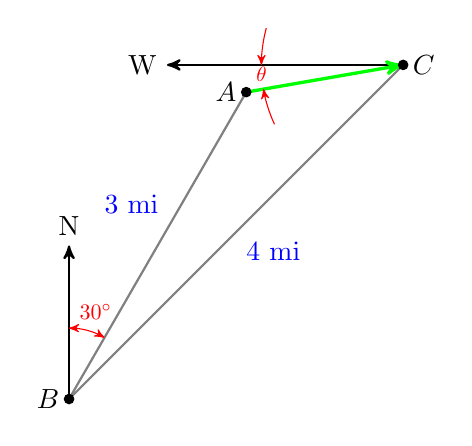
\begin{tikzpicture} [scale=1.5]
\coordinate (B) at (0,0);
\coordinate (A) at (60:3);
\coordinate (C) at (45:4);
\coordinate (N) at (90:1.3);
\draw[black,thick,->,>=stealth'] (B)--(N) node[above]{N};
\draw[black,thick,->,>=stealth'] (C)--++(-2,0) node[left]{W};
\draw[gray,thick] (B)--(A) node[above left, xshift=4, yshift=8, midway, text=blue] {3 mi};
\draw[gray,thick] (B)--(C) node[below right, midway, midway, text=blue] {4 mi};
\draw[green, very thick,->,>=stealth'] (A)--(C);
\draw[red,->,>=stealth'] (C)++(165:1.2) arc(165:180:1.2) node[below, yshift=1.75, scale=.75]{$\theta$};
\draw[red,<-,>=stealth'] (C)++(189.8:1.2) arc(189.8:204.8:1.2);
\draw[red,<->,>=stealth'] (B)++(90:.6) arc(90:60:.6) node[above, midway, xshift=3, yshift=1, scale=.8] {$30\degree$};
\filldraw[black] (B) circle (.04cm) node[left] {$B$};
\filldraw[black] (A) circle (.04cm) node[left] {$A$};
\filldraw[black] (C) circle (.04cm) node[right] {$C$};
\end{tikzpicture}
\newline

fig9-1-4 parallelogram law

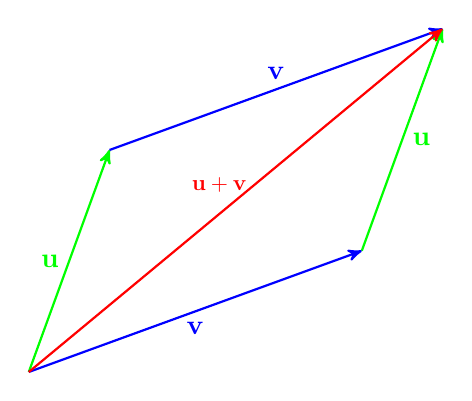
\begin{tikzpicture} [scale=1.5]
\coordinate (O) at (0,0);
\coordinate (A) at (70:2);
\coordinate (B) at (20:3);
\coordinate (C) at ($ (A)+(B) $);
\draw[green,  thick,->,>=stealth'] (O)--++(A) node[left, midway] {\textbf{u}};
\draw[green,  thick,->,>=stealth'] (B)--++(A) node[right, midway] {\textbf{u}};
\draw[blue,  thick,->,>=stealth'] (O)--++(B) node[below, midway] {\textbf{v}};
\draw[blue,  thick,->,>=stealth'] (A)--++(B) node[above, midway] {\textbf{v}};
\draw[red,  thick,->,>=stealth'] (O)--++($ (A)+(B)$) node[above, midway, xshift=-6, scale=.8] {$\textbf{u}+\textbf{v}$};

\end{tikzpicture}
\newline

fig9-1-5 beetle on conveyor belt

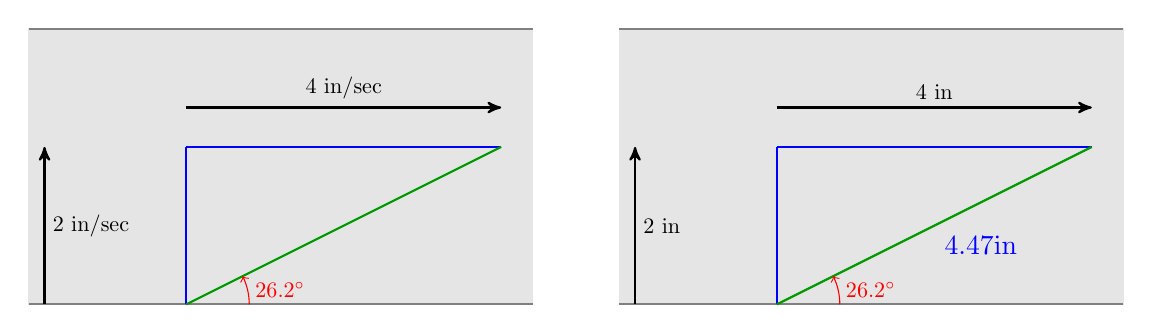
\begin{tikzpicture}
\coordinate (O) at (0,0);
\coordinate (A) at (0,2);
\coordinate (B) at (4,0);
\filldraw[lightgray!40] (-2,0) rectangle ++(6.4,3.5);
\draw[gray,thick] (-2,0) --++(6.4,0);
\draw[gray,thick] (-2,3.5) --++(6.4,0);
\draw[blue,thick] (O)--(A);
\draw[blue,thick] (A) --++(B);
\draw[green!60!black,thick] (O)--($ (A)+(B) $);
\draw[red, ->] (0:.8) arc(0:{atan(1/2)}:0.8) node[right, midway, yshift=0, scale=.8] {$26.2\degree$};
\draw[black,thick,->,>=stealth'] ($(O)+(-1.8,0)$)--++(0,2) node[right,midway, scale=.8] {2 in/sec};
\draw[black,thick,->,>=stealth'] ($(O)+(0,2.5)$)--++(4,0) node[above,midway, scale=.8] {4 in/sec};

\coordinate (O) at (7.5,0);
\coordinate (A) at ($(O)+(0,2)$);
\coordinate (B) at ($(O)+(4,0)$);
\filldraw[lightgray!40] ($ (O)+(-2,0)$) rectangle ++(6.4,3.5);
\draw[gray,thick] ($(O)+(-2,0)$) --++(6.4,0);
\draw[gray,thick] ($(O)+(-2,3.5)$) --++(6.4,0);
\draw[blue,thick] (O)--(A);
\draw[blue,thick] (A) --++(4,0);
\draw[green!60!black,thick] (O)--($ (A)+(4,0) $) node[below right, midway, text=blue] {4.47in};
\draw[red, ->] ($(O)+(0:.8)$) arc(0:{atan(1/2)}:0.8) node[right, midway, yshift=0, scale=.8] {$26.2\degree$};
\draw[black,thick,->,>=stealth'] ($(O)+(-1.8,0)$)--++(0,2) node[right,midway, scale=.8] {2 in};
\draw[black,thick,->,>=stealth'] ($(O)+(0,2.5)$)--++(4,0) node[above,midway, scale=.8] {4 in};

\end{tikzpicture}
\newline


exam9-1-6ans velocity vectors

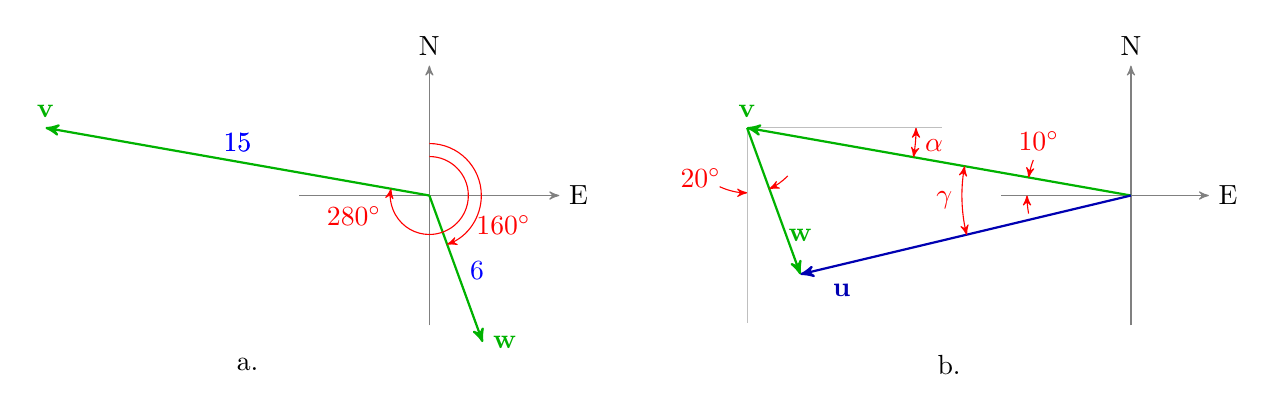
\begin{tikzpicture} [scale=.33]
\coordinate (O) at (0,0);
\draw[gray,->,>=stealth'] (0,-5) --++(0,10) node[above, text=black]{N};
\draw[gray,->,>=stealth'] (-5,0) --++(10,0) node[right, text=black]{E};
\draw[green!70!black,thick,->,>=stealth'] (O) --++(170:15) node[above]{\textbf{v}};
\node[above, text=blue] at (170:7.5) {15};
\draw[green!70!black,thick,->,>=stealth'] (O) --++(-70:6) node[right]{\textbf{w}};
\node[above right, yshift=-3, text=blue] at (-70:3.5) {6};
\draw[red,->,>=stealth'] (0,2) arc(90:-70:2) node[below right, xshift=-5, yshift=-7, midway]{$160\degree$};
\draw[red,->,>=stealth'] (0,1.5) arc(90:-190:1.5) node[left, xshift=0, yshift=-10]{$280\degree$};
\node at (-7,-6.5) {a.};

%second diagram
\def\delx{27};
\coordinate (O) at (\delx,0);
\draw[gray,->,>=stealth'] ($ (O)+(0,-5)$) --++(0,10) node[above, text=black]{N};
\draw[gray,->,>=stealth'] ($ (O)+(-5,0)$) --++(8,0) node[right, text=black]{E};
\coordinate (P) at ($ (O) +(170:15)$);
\draw[lightgray] (P)--++(7.5,0);
\draw[lightgray] (P)--++(0,-7.5);
\draw[green!70!black,thick,->,>=stealth'] (O) --(P) node[above]{\textbf{v}};
\node[above, text=blue] at (170:7.5) {15};
\draw[green!70!black,thick,->,>=stealth'] ($(O)+(170:15) $) --++(-70:6) node[above , yshift=8]{\textbf{w}};
\draw[blue!70!black,thick,->,>=stealth'] (O) --++($(-70:6)+(170:15) $)node[below right, xshift=8]{\textbf{u}};
\draw[red,<-,>=stealth'] ($ (P)+(0,-2.5)$) arc(-90:-115:2.5) node[left, xshift=4,yshift=3] {$20\degree$};
\draw[red,<-,>=stealth'] ($ (P)+(-70:2.5)$) arc(-65:-45:2.5);
\draw[red,<->,>=stealth'] ($ (P)+(6.5,0)$) arc(0:-10:6.5) node[right, midway, yshift=-1] {$\alpha$};
\draw[red,<-,>=stealth'] ($ (O)+(-4.,0)$) arc(180:190:4.);
\draw[red,<-,>=stealth'] ($ (O)+(170:4.)$) arc(170:160:4.) node[above, xshift=2] {$10\degree$};
\draw[red,<->,>=stealth'] ($ (O)+(170:6.5)$) arc(170:193.5:6.5) node[left, midway] {$\gamma$};
\node at ($(O)+(-7,-6.5)$) {b.};
\end{tikzpicture}


exam9-1-7ans  velocity vectors

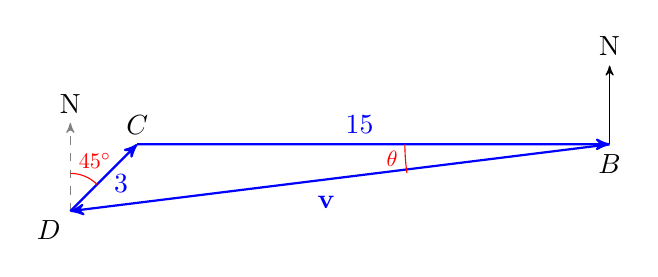
\begin{tikzpicture} [scale=.4]
\coordinate (D) at (0,0);
\coordinate (C) at (45:3);
\coordinate (B) at ($ (C) + (15,0) $);
\draw[gray,dashed,->,>=stealth'] (D)--++(0,2.8) node[above, text=black]{N};
\draw[black,->,>=stealth'] (B)--++(0,2.5) node[above]{N};
\draw[blue,thick, ->,>=stealth'] (D) -- (C) node[right, yshift=-2, midway] {3};
\draw[blue,thick,->,>=stealth'] (C)--(B) node[above,midway, xshift=-5] {15};
\draw[blue,thick,->,>=stealth'] (B)--(D) node[below,midway, xshift=-5, yshift=-3] {\textbf{v}};
\draw[red] (0,1.2) arc(90:45:1.2) node[above right, xshift=-5, midway, scale=.8]{$45\degree$};
\draw[red] ($ (B) + (-6.5,0) $) arc(180:188.1:6.5) node[left, midway, yshift=0, scale=.8]{$\theta$};
\node[below left] at (D) {$D$};
\node[above] at (C) {$C$};
\node[below] at (B) {$B$};
\end{tikzpicture}
\newline


fig9-1-6  velocity vectors

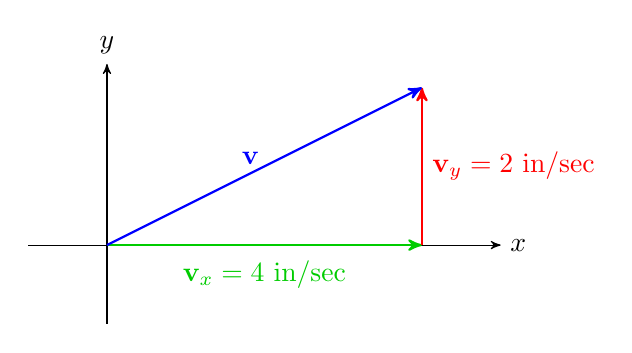
\begin{tikzpicture} 
\coordinate (O) at (0,0);
\coordinate (x) at (4,0);
\coordinate (v) at (4,2);
\draw[black,->,>=stealth'] (0,-1)--(0,2.3) node[above]{$y$};
\draw[black,->,>=stealth'] (-1,0)--(5,0) node[right]{$x$};
\draw[green!80!black,thick, ->,>=stealth'] (O) -- (x) node[below,midway, yshift=-2] {$\textbf{v}_x=4$  in/sec};
\draw[red,thick,->,>=stealth'] (x)--(v) node[right,midway]  {$\textbf{v}_y=2$ in/sec};
\draw[blue,thick,->,>=stealth'] (O)--(v) node[above,midway, xshift=-5, yshift=-3] {\textbf{v}};
\end{tikzpicture}
\newline


fig9-1-7 four quadrants

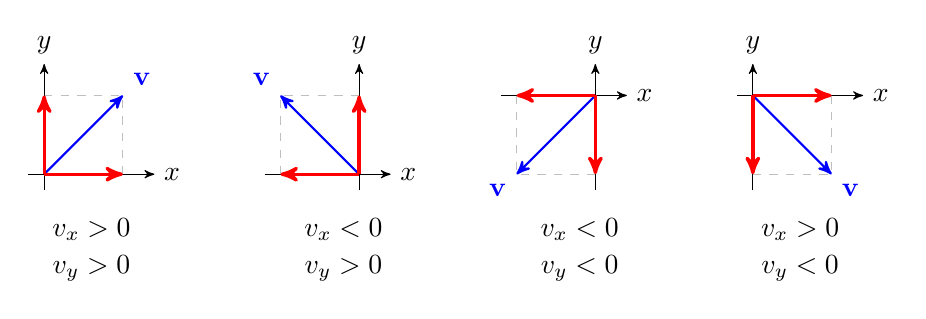
\begin{tikzpicture}
\coordinate(O) at (0,0);
\coordinate(x) at ($ (O) + (1,0) $);
\coordinate(y) at ($ (O) + (0,1) $);
\coordinate(v) at ($ (O) + (1,1) $);
\draw[lightgray,dashed] (y)--(v)--(x);
\draw[black, ->,>=stealth'] (O)++(-0.2,0)--++(1.6,0) node[right]{$x$};
\draw[black, ->,>=stealth'] (O)++(0,-0.2)--++(0,1.6) node[above]{$y$};
\draw[blue,thick,->,>=stealth'] (O)--(v) node[above right]{\textbf{v}};
\draw[red, very thick,->,>=stealth'] (O)--(x);
\draw[red, very thick,->,>=stealth'] (O)--(y);
\node at ($ (O) + (.6,-.7) $) {$v_x > 0$};
\node at ($ (O) + (.6,-1.2) $) {$v_y > 0$};

% second quadrant
\coordinate(O) at (4,0);
\coordinate(x) at ($ (O) + (-1,0) $);
\coordinate(y) at ($ (O) + (0,1) $);
\coordinate(v) at ($ (O) + (-1,1) $);
\draw[lightgray,dashed] (y)--(v)--(x);
\draw[black, ->,>=stealth'] (O)++(-1.2,0)--++(1.6,0) node[right]{$x$};
\draw[black, ->,>=stealth'] (O)++(0,-0.2)--++(0,1.6) node[above]{$y$};
\draw[blue,thick,->,>=stealth'] (O)--(v) node[above left]{\textbf{v}};
\draw[red, very thick,->,>=stealth'] (O)--(x);
\draw[red, very thick,->,>=stealth'] (O)--(y);
\node at ($ (O) + (-.2,-.7) $) {$v_x < 0$};
\node at ($ (O) + (-.2,-1.2) $) {$v_y > 0$};

% third quadrant
\coordinate(O) at (7,1);
\coordinate(x) at ($ (O) + (-1,0) $);
\coordinate(y) at ($ (O) + (0,-1) $);
\coordinate(v) at ($ (O) + (-1,-1) $);
\draw[lightgray,dashed] (y)--(v)--(x);
\draw[black, ->,>=stealth'] (O)++(-1.2,0)--++(1.6,0) node[right]{$x$};
\draw[black, ->,>=stealth'] (O)++(0,-1.2)--++(0,1.6) node[above]{$y$};
\draw[blue,thick,->,>=stealth'] (O)--(v) node[below left]{\textbf{v}};
\draw[red, very thick,->,>=stealth'] (O)--(x);
\draw[red, very thick,->,>=stealth'] (O)--(y);
\node at ($ (O) + (-.2,-1.7) $) {$v_x < 0$};
\node at ($ (O) + (-.2,-2.2) $) {$v_y < 0$};

% third quadrant
\coordinate(O) at (9,1);
\coordinate(x) at ($ (O) + (1,0) $);
\coordinate(y) at ($ (O) + (0,-1) $);
\coordinate(v) at ($ (O) + (1,-1) $);
\draw[lightgray,dashed] (y)--(v)--(x);
\draw[black, ->,>=stealth'] (O)++(-.2,0)--++(1.6,0) node[right]{$x$};
\draw[black, ->,>=stealth'] (O)++(0,-1.2)--++(0,1.6) node[above]{$y$};
\draw[blue,thick,->,>=stealth'] (O)--(v) node[below right]{\textbf{v}};
\draw[red, very thick,->,>=stealth'] (O)--(x);
\draw[red, very thick,->,>=stealth'] (O)--(y);
\node at ($ (O) + (.6,-1.7) $) {$v_x > 0$};
\node at ($ (O) + (.6,-2.2) $) {$v_y < 0$};

\end{tikzpicture}
\newline


exam9-1-8ans  velocity vectors

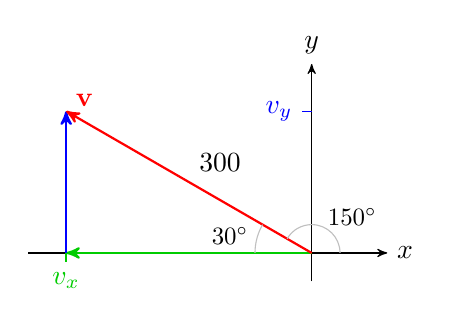
\begin{tikzpicture} [scale=1.2]
\coordinate (O) at (0,0);
\coordinate (x) at ($ 3*cos(150)*(1,0)$);
\coordinate (y) at ($ 3*sin(150)*(0,1)$);
\coordinate (v) at (150:3);
\draw[black,->,>=stealth'] (0,-.3)--(0,2) node[above]{$y$};
\draw[black,->,>=stealth'] (-3,0)--(.8,0) node[right]{$x$};
\draw[green!80!black,thick, ->,>=stealth'] (O) -- (x) ;
\draw[green!80!black,thick] (x) -- ++(0,-0.1) node[below] {$v_x$};
\draw[blue,thick,->,>=stealth'] (x)--(v);
\draw[red,thick,->,>=stealth'] (O)--(v) node[above right,midway, text=black] {300};
\node[above right, yshift=-2, text=red] at (v) {\textbf{v}};
\draw[lightgray] (.3,0) arc(0:150:0.3) node[above right, midway, yshift=-3, text=black, scale=.9]{$150\degree$};
\draw[lightgray] (-.6,0) arc(180:150:0.6) node[left, midway, yshift=1, text=black, scale=.9]{$30\degree$};
\draw[blue] (y)--++(-0.1,0) node[left]{$v_y$};
\end{tikzpicture}
\newline

exam9-1-9ans velocity vectors

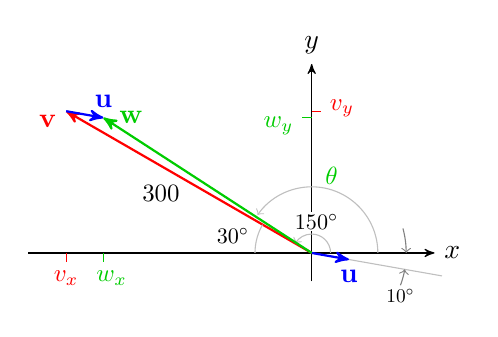
\begin{tikzpicture} [scale=1.2]
\coordinate (O) at (0,0);
\coordinate (x) at ($ 3*cos(150)*(1,0)$);
\coordinate (y) at ($ 3*sin(150)*(0,1)$);
\coordinate (v) at (150:3);
\coordinate (u) at (-10:0.4);
\coordinate (wx) at ($ 3*cos(150)*(1,0) + .4*cos(-10)*(1,0) $);
\coordinate (wy) at ($ 3*sin(150)*(0,1) + .4*sin(-10)*(0,1) $);
\draw[black,->,>=stealth'] (0,-.3)--(0,2) node[above]{$y$};
\draw[black,->,>=stealth'] (-3,0)--(1.3,0) node[right]{$x$};
\draw[red,thick,->,>=stealth'] (O)--(v) node[below left,midway, yshift=2, text=black, scale=.9] {300};
\node[below left, yshift=2, text=red] at (v) {\textbf{v}};
\draw[lightgray] (O)--($ 3.5*(u) $);
\draw[blue,thick,->,>=stealth'] (O)--++(u) node[below]{\textbf{u}};
\draw[blue,thick,->,>=stealth'] (v)--++(u) node[above]{\textbf{u}};

\draw[lightgray, ->] (.2,0) arc(0:150:0.2) node[above, midway, yshift=1, text=black, scale=.8, fill=white, inner sep=1]{$150\degree$};
\draw[lightgray] (-.6,0) arc(180:150:0.6) node[left, midway, yshift=1, text=black, scale=.8]{$30\degree$};
\draw[green!80!black,thick,->,>=stealth'] (O)--($ (v)+(u) $) node[right, xshift=2]{\textbf{w}};

\draw[gray, <-] (1,0) arc(0:15:1);
\draw[gray, <-] (-10:1) arc(-10:-20:1) node[below, yshift=1, text=black, scale=.7]{$10\degree$};
\draw[lightgray, ->] (.7,0) arc(0:145:0.7) node[above, midway, yshift=1, text=green!80!black, fill=white, inner sep=1, scale=.9]{$\theta$};

\draw[red] (y)--++(0.1,0) node[right, yshift=1, scale=.9]{$v_y$};
\draw[red] (x) -- ++(0,-0.1) node[below, scale=.9] {$v_x$};
\draw[green!80!black] (wy)--++(-0.1,0) node[left, yshift=-3, scale=.9]{$w_y$};
\draw[green!80!black] (wx) -- ++(0,-0.1) node[below, xshift=3, scale=.9] {$w_x$};
\end{tikzpicture}
\newline

hp9-1-1ans position vector

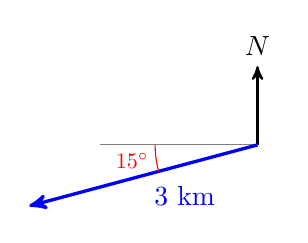
\begin{tikzpicture}
\draw[black,thick,->,>=stealth'] (0,0)--(0,1) node[above]{$N$};
\draw[gray] (0,0) --(-2,0);
\draw[blue, very thick,->,>=stealth'] (0,0)--(195:3) node[below right, midway] {3 km};
\draw[red] (-1.3,0) arc(180:195:1.3) node[left, midway, yshift=-1, scale=.8] {$15\degree$};
\end{tikzpicture}
\newline

hp9-1-3ans velocity vector

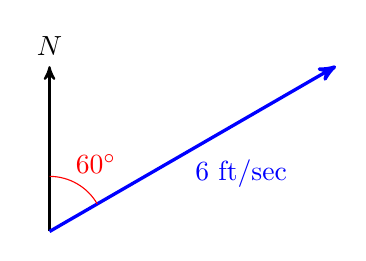
\begin{tikzpicture} [scale=.7]
\draw[black,thick,->,>=stealth'] (0,0)--(0,3) node[above]{$N$};
\draw[blue, very thick,->,>=stealth'] (0,0)--(30:6) node[below right, midway, xshift=-3] {6 ft/sec};
\draw[red] (0,1) arc(90:30:1) node[above right, midway, xshift=-4] {$60\degree$};
\end{tikzpicture}
\newline


hp9-1-5ans velocity vector

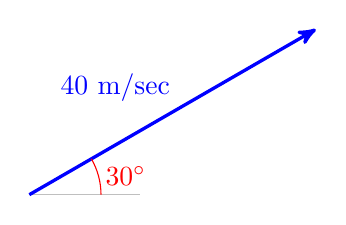
\begin{tikzpicture} [scale=.7]
\draw[lightgray] (0,0)--(2,0);
\draw[blue, very thick,->,>=stealth'] (0,0)--(30:6) node[above left, midway, xshift=3] {40 m/sec};
\draw[red] (1.3,0) arc(0:30:1.3) node[right, midway, xshift=-1] {$30\degree$};
\end{tikzpicture}
\newline

hp9-1-7 vectors on grid

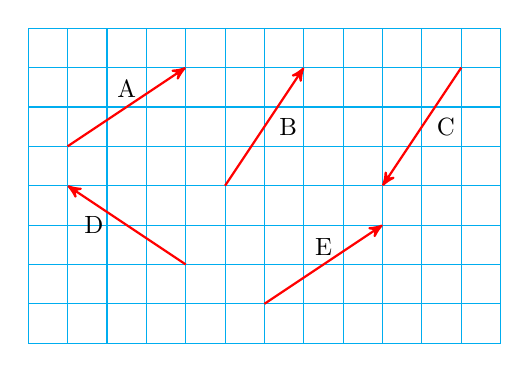
\begin{tikzpicture} [scale=.5]
\draw[cyan] (0,0) grid (12,8);
\draw[red,thick,->,>=stealth'] (1,5)--++(3,2) node[above, midway, text=black, scale=.9]{A};
\draw[red,thick,->,>=stealth'] (5,4)--++(2,3) node[right, midway, xshift=2, text=black, scale=.9]{B};
\draw[red,thick,->,>=stealth'] (11,7)--++(-2,-3) node[right, midway, xshift=2, text=black, scale=.9]{C};
\draw[red,thick,->,>=stealth'] (4,2)--++(-3,2) node[left, midway, xshift=-5, text=black, scale=.9]{D};
\draw[red,thick,->,>=stealth'] (6,1)--++(3,2) node[above, midway, text=black, scale=.9]{E};

\end{tikzpicture}
\newline


hp9-1-8 vectors on grid

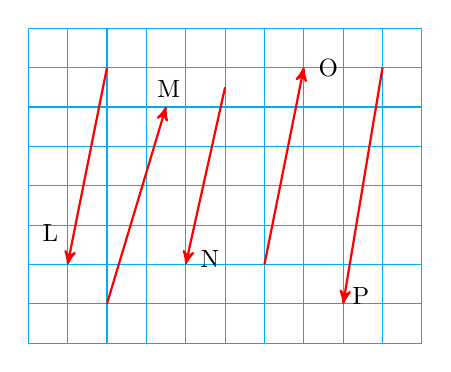
\begin{tikzpicture} [scale=.5]
\draw[cyan] (0,0) grid (10,8);
\draw[red,thick,->,>=stealth'] (2,7)--++(-1,-5) node[above left, yshift=5, text=black, scale=.9]{L};
\draw[red,thick,->,>=stealth'] (2,1)--++(1.5,5) node[above, xshift=1, text=black, scale=.9]{M};
\draw[red,thick,->,>=stealth'] (5,6.5)--++(-1,-4.5) node[right, yshift=2, xshift=2, text=black, scale=.9]{N};
\draw[red,thick,->,>=stealth'] (6,2)--++(1,5) node[right,  xshift=2, text=black, scale=.9]{O};
\draw[red,thick,->,>=stealth'] (9,7)--++(-1,-6) node[right, yshift=3, text=black, scale=.9]{P};

\end{tikzpicture}
\newline


hp9-1-9 vectors on grid

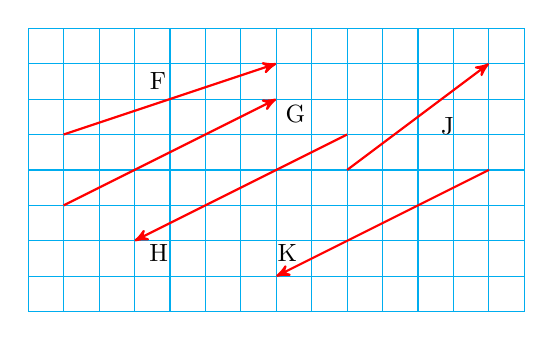
\begin{tikzpicture} [scale=.45]
\draw[cyan] (0,0) grid (14,8);
\draw[red,thick,->,>=stealth'] (1,5)--++(6,2) node[above left, midway, xshift=2, text=black, scale=.9]{F};
\draw[red,thick,->,>=stealth'] (1,3)--++(6,3) node[below right, yshift=1, text=black, scale=.9]{G};
\draw[red,thick,->,>=stealth'] (9,5)--++(-6,-3) node[below right, xshift=2, yshift=2, text=black, scale=.9]{H};
\draw[red,thick,->,>=stealth'] (9,4)--++(4,3) node[below right, midway,  xshift=5, yshift=3, text=black, scale=.9]{J};
\draw[red,thick,->,>=stealth'] (13,4)--++(-6,-3) node[above, yshift=2, xshift=4, text=black, scale=.9]{K};

\end{tikzpicture}
\newline


hp9-1-10 vectors on grid

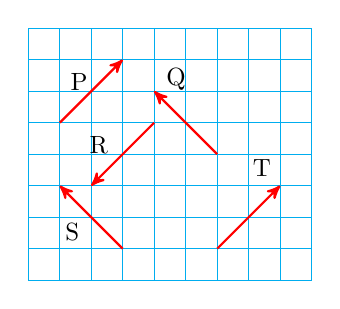
\begin{tikzpicture} [scale=.4]
\draw[cyan] (0,0) grid (9,8);
\draw[red,thick,->,>=stealth'] (1,5)--++(2,2) node[above left, midway, xshift=2, yshift=-3, text=black, scale=.9]{P};
\draw[red,thick,->,>=stealth'] (6,4)--++(-2,2) node[above right, xshift=1, yshift=-3, text=black, scale=.9]{Q};
\draw[red,thick,->,>=stealth'] (4,5)--++(-2,-2) node[above left, midway, xshift=-2, yshift=-3, text=black, scale=.9]{R};
\draw[red,thick,->,>=stealth'] (3,1)--++(-2,2) node[below left, midway,  xshift=-1, yshift=1, text=black, scale=.9]{S};
\draw[red,thick,->,>=stealth'] (6,1)--++(2,2) node[above left,  text=black, scale=.9]{T};

\end{tikzpicture}
\newline



hp9-1-11 vectors on grid

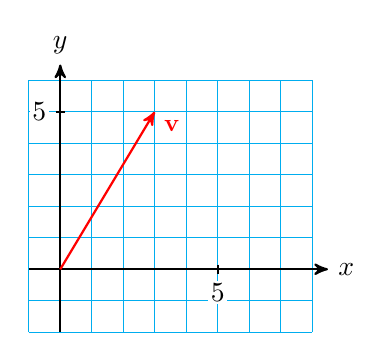
\begin{tikzpicture} [scale=.4]
\draw[cyan] (-1,-2) grid (8,6);
\draw[black,thick,->,>=stealth'] (-1,0)--(8.5,0) node[right] {$x$};
\draw[black,thick,->,>=stealth'] (0,-2)--(0,6.5) node[above] {$y$};
\foreach \x in {5} {
 \draw[black,thick] (\x,.15)--++(0,-.3) node[below, yshift=-2, fill=white, inner sep=1] {$\x$};
 \draw[black,thick] (.15,\x)--++(-.3,0) node[left, xshift=-2, fill=white, inner sep=1] {$\x$};
};

\draw[red,thick,->,>=stealth'] (0,0)--++(3,5) node[right, yshift=-2, yshift=-3, scale=.9]{\textbf{v}};

\end{tikzpicture}
\newline



hp9-1-11ans vectors on grid

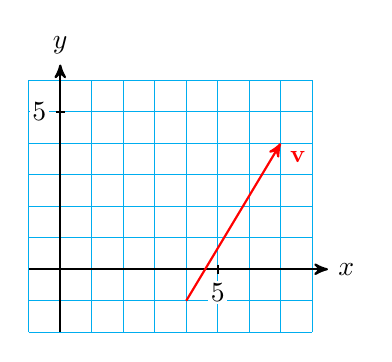
\begin{tikzpicture} [scale=.4]
\draw[cyan] (-1,-2) grid (8,6);
\draw[black,thick,->,>=stealth'] (-1,0)--(8.5,0) node[right] {$x$};
\draw[black,thick,->,>=stealth'] (0,-2)--(0,6.5) node[above] {$y$};
\foreach \x in {5} {
 \draw[black,thick] (\x,.15)--++(0,-.3) node[below, yshift=-2, fill=white, inner sep=1] {$\x$};
 \draw[black,thick] (.15,\x)--++(-.3,0) node[left, xshift=-2, fill=white, inner sep=1] {$\x$};
};

\draw[red,thick,->,>=stealth'] (4,-1)--++(3,5) node[right, yshift=-2, yshift=-3, scale=.9]{\textbf{v}};

\end{tikzpicture}
\newline



hp9-1-12 vectors on grid

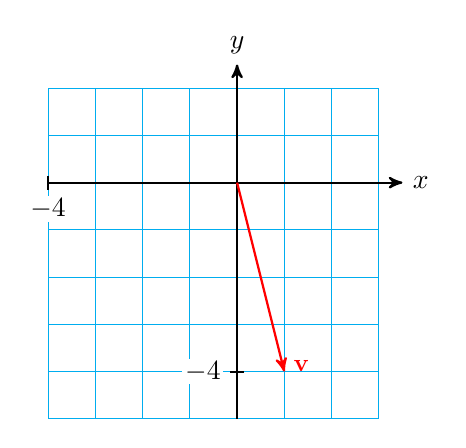
\begin{tikzpicture} [scale=.6]
\draw[cyan] (-4,-5) grid (3,2);
\draw[black,thick,->,>=stealth'] (-4,0)--(3.5,0) node[right] {$x$};
\draw[black,thick,->,>=stealth'] (0,-5)--(0,2.5) node[above] {$y$};
\foreach \x in {-4} {
 \draw[black,thick] (\x,.15)--++(0,-.3) node[below, yshift=-2, fill=white, inner sep=1] {$\x$};
 \draw[black,thick] (.15,\x)--++(-.3,0) node[left, xshift=-2, fill=white, inner sep=1] {$\x$};
};

\draw[red,thick,->,>=stealth'] (0,0)--++(1,-4) node[right, yshift=2,  scale=.9]{\textbf{v}};

\end{tikzpicture}
\newline



hp9-1-13 vector on grid

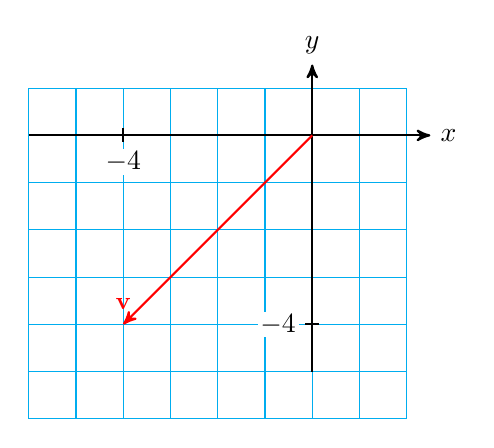
\begin{tikzpicture} [scale=.6]
\draw[cyan] (-6,-6) grid (2,1);
\draw[black,thick,->,>=stealth'] (-6,0)--(2.5,0) node[right] {$x$};
\draw[black,thick,->,>=stealth'] (0,-5)--(0,1.5) node[above] {$y$};
\foreach \x in {-4} {
 \draw[black,thick] (\x,.15)--++(0,-.3) node[below, yshift=-2, fill=white, inner sep=1] {$\x$};
 \draw[black,thick] (.15,\x)--++(-.3,0) node[left, xshift=-2, fill=white, inner sep=1] {$\x$};
};

\draw[red,thick,->,>=stealth'] (0,0)--++(-4,-4) node[above, yshift=2,  scale=.9]{\textbf{v}};

\end{tikzpicture}
\newline



hp9-1-13ans vector on grid

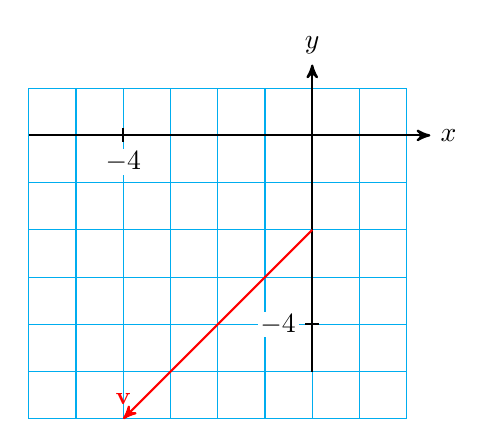
\begin{tikzpicture} [scale=.6]
\draw[cyan] (-6,-6) grid (2,1);
\draw[black,thick,->,>=stealth'] (-6,0)--(2.5,0) node[right] {$x$};
\draw[black,thick,->,>=stealth'] (0,-5)--(0,1.5) node[above] {$y$};
\foreach \x in {-4} {
 \draw[black,thick] (\x,.15)--++(0,-.3) node[below, yshift=-2, fill=white, inner sep=1] {$\x$};
 \draw[black,thick] (.15,\x)--++(-.3,0) node[left, xshift=-2, fill=white, inner sep=1] {$\x$};
};

\draw[red,thick,->,>=stealth'] (0,-2)--++(-4,-4) node[above, yshift=2,  scale=.9]{\textbf{v}};

\end{tikzpicture}
\newline



hp9-1-14 vector on grid

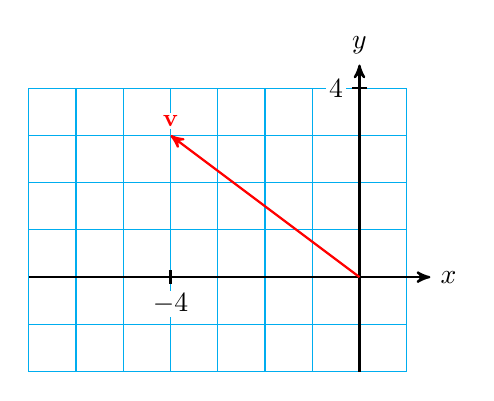
\begin{tikzpicture} [scale=.6]
\draw[cyan] (-7,-2) grid (1,4);
\draw[black,thick,->,>=stealth'] (-7,0)--(1.5,0) node[right] {$x$};
\draw[black,thick,->,>=stealth'] (0,-2)--(0,4.5) node[above] {$y$};
\foreach \x in {4} {
 \draw[black,thick] (-\x,.15)--++(0,-.3) node[below, yshift=-2, fill=white, inner sep=1] {$-\x$};
 \draw[black,thick] (.15,\x)--++(-.3,0) node[left, xshift=-2, fill=white, inner sep=1] {$\x$};
};

\draw[red,thick,->,>=stealth'] (0,0)--++(-4,3) node[above, yshift=2,  scale=.9, fill=white, inner sep=1]{\textbf{v}};

\end{tikzpicture}
\newline



hp9-1-15 vector on grid

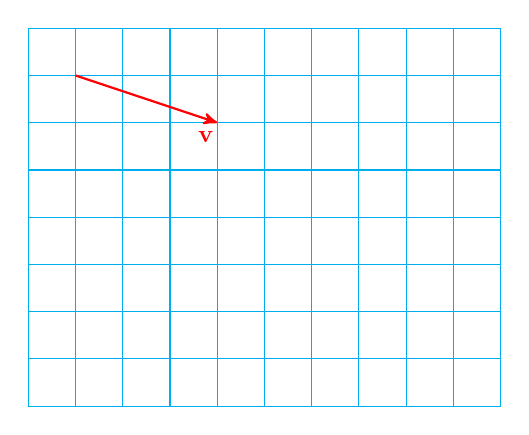
\begin{tikzpicture} [scale=.6]
\draw[cyan] (0,0) grid (10,8);
\coordinate (v) at (3,-1);

\draw[red,thick,->,>=stealth'] (1,7)--++(v) node[below left, yshift=-2,  scale=.9, fill=white, inner sep=1]{\textbf{v}};

\end{tikzpicture}
\newline



hp9-1-15ans vectors on grid

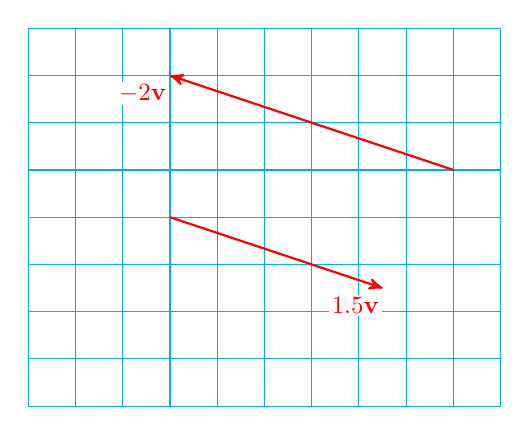
\begin{tikzpicture} [scale=.6]
\draw[cyan] (0,0) grid (10,8);
\coordinate (v) at (3,-1);
\coordinate (vn2) at ($ -2*(v) $);
\coordinate (v15) at ($ 1.5*(v) $);

\draw[red,thick,->,>=stealth'] (9,5)--++(vn2) node[below left, yshift=-2,  scale=.9, fill=white, inner sep=1]{$-2$\textbf{v}};
\draw[red,thick,->,>=stealth'] (3,4)--++(v15) node[below left, yshift=-2,  scale=.9, fill=white, inner sep=1]{$1.5$\textbf{v}};

\end{tikzpicture}
\newline



hp9-1-16 vector on grid

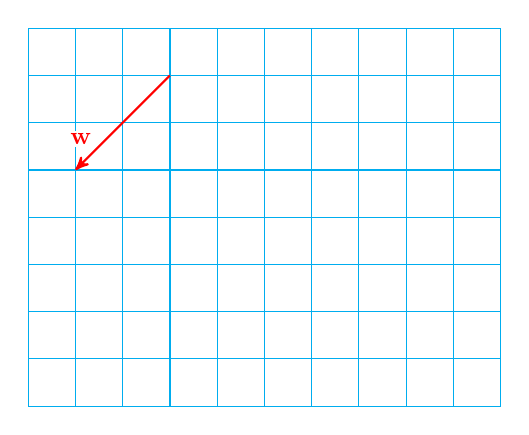
\begin{tikzpicture} [scale=.6]
\draw[cyan] (0,0) grid (10,8);
\coordinate (w) at (-2,-2);

\draw[red,thick,->,>=stealth'] (3,7)--++(w) node[above, xshift=2 , yshift=8,  scale=.9, fill=white, inner sep=1]{\textbf{w}};

\end{tikzpicture}
\newline



hp9-1-17 vector on grid

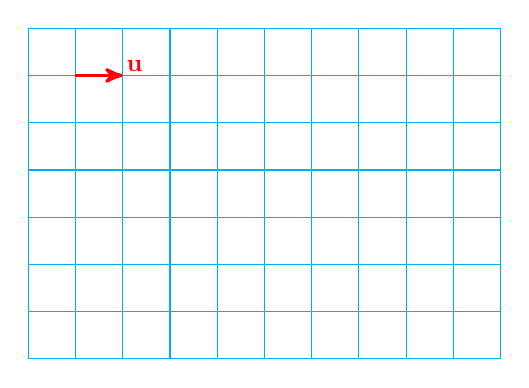
\begin{tikzpicture} [scale=.6]
\draw[cyan] (0,0) grid (10,7);
\coordinate (u) at (1,0);

\draw[red,very thick,->,>=stealth'] (1,6)--++(u) node[above right, scale=.9, fill=white, inner sep=1]{\textbf{u}};

\end{tikzpicture}
\newline



hp9-1-17ans vector on grid

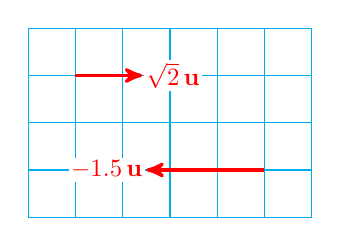
\begin{tikzpicture} [scale=.6]
\draw[cyan] (0,0) grid (6,4);
\coordinate (u) at (1,0);

\draw[red,very thick,->,>=stealth'] (5,1)--++($-2.5*(u)$) node[left, scale=.9, fill=white, inner sep=1]{$-1.5\,$\textbf{u}};
\draw[red,very thick,->,>=stealth'] (1,3)--++($sqrt(2)*(u)$) node[right, scale=.9, fill=white, inner sep=1]{$\sqrt{2}\,$\textbf{u}};

\end{tikzpicture}
\newline



hp9-1-18 vector on grid

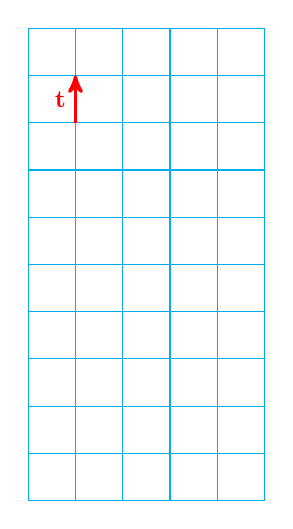
\begin{tikzpicture} [scale=.6]
\draw[cyan] (0,0) grid (5,10);
\coordinate (t) at (0,1);

\draw[red,very thick,->,>=stealth'] (1,8)--++(t) node[left, midway, xshift=-2, scale=.9, fill=white, inner sep=1]{\textbf{t}};

\end{tikzpicture}
\newline


hp9-1-19 vectors on grid

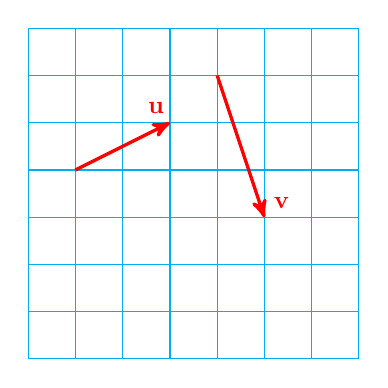
\begin{tikzpicture} [scale=.6]
\draw[cyan] (0,0) grid (7,7);
\coordinate (u) at (2,1);
\coordinate (v) at (1,-3);

\draw[red,very thick,->,>=stealth'] (1,4)--++(u) node[above, xshift=-5, yshift=2, scale=.9, fill=white, inner sep=1]{\textbf{u}};
\draw[red,very thick,->,>=stealth'] (4,6)--++(v) node[right, xshift=2, yshift=5, scale=.9, fill=white, inner sep=1]{\textbf{v}};

\end{tikzpicture}
\newline


hp9-1-19ans vectors on grid

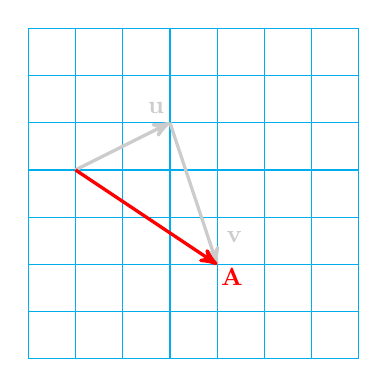
\begin{tikzpicture} [scale=.6]
\draw[cyan] (0,0) grid (7,7);
\coordinate (u) at (2,1);
\coordinate (v) at (1,-3);
\coordinate (A) at (3,-2);

\draw[lightgray!80!white,very thick,->,>=stealth'] (1,4)--++(u) node[above, xshift=-5, yshift=2, scale=.9, fill=white, inner sep=1]{\textbf{u}};
\draw[lightgray!80!white,very thick,->,>=stealth'] (3,5)--++(v) node[right, xshift=2, yshift=10, scale=.9, fill=white, inner sep=1]{\textbf{v}};
\draw[red,very thick,->,>=stealth'] (1,4)--++(A) node[below right,  scale=.9, fill=white, inner sep=1]{\textbf{A}};

\end{tikzpicture}
\newline


hp9-1-20 vectors on grid

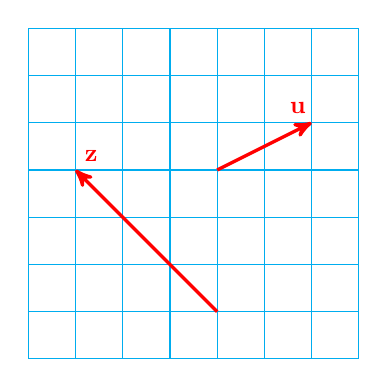
\begin{tikzpicture} [scale=.6]
\draw[cyan] (0,0) grid (7,7);
\coordinate (u) at (2,1);
\coordinate (z) at (-3,3);

\draw[red,very thick,->,>=stealth'] (4,4)--++(u) node[above, xshift=-5, yshift=2, scale=.9, fill=white, inner sep=1]{\textbf{u}};
\draw[red,very thick,->,>=stealth'] (4,1)--++(z) node[right, xshift=2, yshift=5, scale=.9, fill=white, inner sep=1]{\textbf{z}};

\end{tikzpicture}
\newline


hp9-1-21 vectors on grid

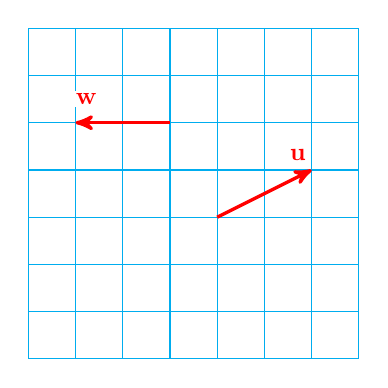
\begin{tikzpicture} [scale=.6]
\draw[cyan] (0,0) grid (7,7);
\coordinate (u) at (2,1);
\coordinate (w) at (-2,0);

\draw[red,very thick,->,>=stealth'] (4,3)--++(u) node[above, xshift=-5, yshift=2, scale=.9, fill=white, inner sep=1]{\textbf{u}};
\draw[red,very thick,->,>=stealth'] (3,5)--++(w) node[above, xshift=4, yshift=5, scale=.9, fill=white, inner sep=1]{\textbf{w}};

\end{tikzpicture}
\newline


hp9-1-21ans vectors on grid

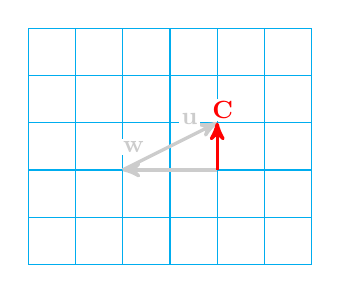
\begin{tikzpicture} [scale=.6]
\draw[cyan] (1,0) grid (7,5);
\coordinate (u) at (2,1);
\coordinate (w) at (-2,0);
\coordinate (C) at (0,1);

\draw[lightgray!80!white,very thick,->,>=stealth'] (3,2)--++(u) node[above, xshift=-10, yshift=-2, scale=.9, fill=white, inner sep=1]{\textbf{u}};
\draw[lightgray!80!white,very thick,->,>=stealth'] (5,2)--++(w) node[above, xshift=4, yshift=5, scale=.9, fill=white, inner sep=1]{\textbf{w}};
\draw[red,very thick,->,>=stealth'] (5,2)--++(C) node[above, xshift=2,  scale=.9, fill=white, inner sep=1]{\textbf{C}};

\end{tikzpicture}
\newline


hp9-1-22 vectors on grid

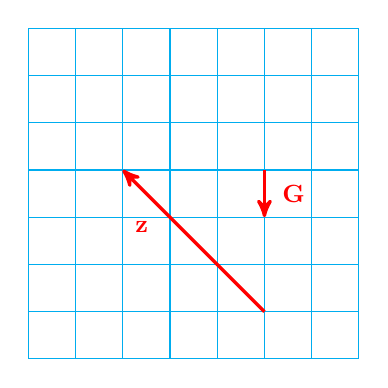
\begin{tikzpicture} [scale=.6]
\draw[cyan] (0,0) grid (7,7);
\coordinate (G) at (0,-1);
\coordinate (z) at (-3,3);

\draw[red,very thick,->,>=stealth'] (5,4)--++(G) node[right, midway, xshift=5,  scale=.9, fill=white, inner sep=1]{\textbf{G}};
\draw[red,very thick,->,>=stealth'] (5,1)--++(z) node[left, midway, xshift=-15, yshift=5, scale=.9, fill=white, inner sep=1]{\textbf{z}};

\end{tikzpicture}
\newline


hp9-1-23 vectors on grid

\begin{tikzpicture} [scale=.6]
\draw[cyan] (0,0) grid (7,7);
\coordinate (z) at (-3,3);
\coordinate (F) at (3,2);

\draw[red,very thick,->,>=stealth'] (5,1)--++(z) node[below, xshift=2, yshift=-10, scale=.9, fill=white, inner sep=1]{\textbf{z}};
\draw[red,very thick,->,>=stealth'] (3,4)--++(F) node[below, xshift=-4, yshift=-10, scale=.9, fill=white, inner sep=1]{\textbf{F}};

\end{tikzpicture}
\newline


hp9-1-23ans vectors on grid

\begin{tikzpicture} [scale=.6]
\draw[cyan] (0,0) grid (7,7);
\coordinate (z) at (-3,3);
\coordinate (F) at (3,2);
\coordinate (E) at (0,5);

\draw[lightgray!80!white, thick,->,>=stealth'] (5,1)--++(z) node[below, xshift=2, yshift=-10, scale=.9, fill=white, inner sep=1]{\textbf{z}};
\draw[lightgray!80!white, thick,->,>=stealth'] (2,4)--++(F) node[above, xshift=-15, yshift=-5, scale=.9, fill=white, inner sep=1]{\textbf{F}};
\draw[red,very thick,->,>=stealth'] (5,1)--++(E) node[above, xshift=3,  scale=.9, fill=white, inner sep=1]{\textbf{E}};

\end{tikzpicture}
\newline


hp9-1-24 vectors on grid

\begin{tikzpicture} [scale=.6]
\draw[cyan] (0,0) grid (7,7);
\coordinate (v) at (1,-3);
\coordinate (w) at (-2,0);

\draw[red,very thick,->,>=stealth'] (5,5)--++(v) node[right, xshift=2, yshift=2, scale=.9, fill=white, inner sep=1]{\textbf{v}};
\draw[red,very thick,->,>=stealth'] (4,5)--++(w) node[above, xshift=4, yshift=5, scale=.9, fill=white, inner sep=1]{\textbf{w}};

\end{tikzpicture}
\newline


hp9-1-25 vector on grid

\begin{tikzpicture} [scale=.6]
\draw[cyan] (0,0) grid (7,7);
\coordinate (w) at (-2,0);

\draw[red,very thick,->,>=stealth'] (4,5)--++(w) node[above, xshift=4, yshift=5, scale=.9, fill=white, inner sep=1]{\textbf{w}};

\end{tikzpicture}
\newline


hp9-1-25ans vector on grid

\begin{tikzpicture} [scale=.6]
\draw[cyan] (0,0) grid (7,2);
\coordinate (G) at (-4,0);

\draw[red,very thick,->,>=stealth'] (5,1)--++(G) node[above, xshift=4, yshift=5, scale=.9, fill=white, inner sep=1]{\textbf{G}};

\end{tikzpicture}
\newline


hp9-1-26 vector on grid

\begin{tikzpicture} [scale=.7]
\draw[cyan] (0,0) grid (4,4);
\coordinate (G) at (0,-1);

\draw[red,very thick,->,>=stealth'] (2,3)--++(G) node[right, midway, xshift=5,  scale=.9, fill=white, inner sep=1]{\textbf{G}};

\end{tikzpicture}
\newline


hp9-1-31ans vectors

\begin{tikzpicture} [scale=.1]
\coordinate (v) at (64:45);
\coordinate (w) at (197:32);

\draw[lightgray!80!white,very thick,->,>=stealth'] (0,0)--++(v) node[right, midway, xshift=5,  scale=.9, fill=white, inner sep=1]{45};
\draw[lightgray!80!white,very thick,->,>=stealth'] (v)--++(w) node[above, midway, xshift=-8, scale=.9, fill=white, inner sep=1]{32};
\draw[red,very thick,->,>=stealth'] (0,0)--++($(v)+(w)$) node[left, midway, xshift=-5,  scale=.9, fill=white, inner sep=1]{\textbf{v+w}};

\end{tikzpicture}
\newline


hp9-1-33ans vectors

\begin{tikzpicture} [scale=.5]
\coordinate (v) at (80:8);
\coordinate (w) at (200:13);

\draw[lightgray!80!white,very thick,->,>=stealth'] (0,0)--++(v) node[right, midway, xshift=5,  scale=.9, fill=white, inner sep=1]{8};
\draw[lightgray!80!white,very thick,->,>=stealth'] (v)--++(w) node[above, midway, xshift=-8, scale=.9, fill=white, inner sep=1]{13};
\draw[red,very thick,->,>=stealth'] (0,0)--++($(v)+(w)$) node[below left, midway, xshift=-5,  scale=.9, fill=white, inner sep=1]{\textbf{v+w}};

\end{tikzpicture}
\newline


hp9-1-35ans vectors

\begin{tikzpicture} [scale=.8]
\coordinate (v) at (70:3.6);
\coordinate (w) at (53:0.9);

\draw[lightgray!80!white,very thick,->,>=stealth'] (0,0)--++(v) node[left, midway, xshift=-4,  scale=.9, fill=white, inner sep=1]{3.6};
\draw[lightgray!80!white,very thick,->,>=stealth'] (v)--++(w) node[above left, midway, xshift=-3, scale=.9, fill=white, inner sep=1]{0.9};
\draw[red,very thick,->,>=stealth'] (0,0)--++($(v)+(w)$);

\end{tikzpicture}
\newline


hp9-1-37ans vectors

\begin{tikzpicture} [scale=.04]
\coordinate (v) at (180:103);
\coordinate (w) at (-22:28);
\draw[lightgray!80!white,very thick,->,>=stealth'] (0,0)--++(v) node[below, midway, yshift=-4,  scale=.9, fill=white, inner sep=1]{103};
\draw[lightgray!80!white,very thick,<-,>=stealth'] (v)--++($-1*(w)$) node[below left, midway, xshift=-3, scale=.9, fill=white, inner sep=1]{28};
\draw[red,very thick,->,>=stealth'] (0,0)--++($ -1*(w) + (v)$);

\end{tikzpicture}
\newline


hp9-1-43 vectors on grid

\begin{tikzpicture} [scale=.6]
\draw[cyan] (0,0) grid (7,7);
\coordinate (u) at (2,1);
\coordinate (v) at (1,-3);

\draw[red,very thick,->,>=stealth'] (1,2)--++(u) node[above, xshift=-5, yshift=3, scale=.9, fill=white, inner sep=1]{\textbf{u}};
\draw[red,very thick,->,>=stealth'] (4,4)--++(v) node[right, xshift=4, yshift=5, scale=.9, fill=white, inner sep=1]{\textbf{v}};

\end{tikzpicture}
\newline


hp9-1-43ans vectors on grid

\begin{tikzpicture} [scale=.6]
\draw[cyan] (0,0) grid (7,7);
\coordinate (u) at (2,1);
\coordinate (v) at (1,-3);
\coordinate (A) at ($ (u) - (v) $);

\draw[lightgray!80!white, thick,->,>=stealth'] (1,1)--++(u) node[below, xshift=-5, yshift=-8, scale=.9, fill=white, inner sep=1]{\textbf{u}};
\draw[lightgray!80!white, thick,->,>=stealth'] (3,2)--++($-1*(v)$) node[ right, xshift=8, yshift=-16, scale=.9, fill=white, inner sep=1]{\textbf{-v}};
\draw[red,very thick,->,>=stealth'] (1,1)--++(A) node[above, xshift=3,  scale=.9, fill=white, inner sep=1]{\textbf{A}};

\end{tikzpicture}
\newline




\end{document}
